\documentclass{article}
\usepackage{fancyhdr}
\usepackage{graphicx}
\usepackage{amsmath}
\usepackage{amssymb}
\pagestyle{fancy}

\author{Philipp Kiss}

\lhead{Philipp Kiss}
\rhead{Diskrete Mathematik}

\begin{document}
\pagenumbering{gobble}

\section{test}
\section{Aussagen und Prädikate}
\paragraph{Aussagen} müssen einen distinkten Wahrheitswert haben.
Z.b. \textit{Heute ist es über 10°C}. Ein ambiger Term wie \(x+3=5\) ist keine Aussage, da der Wahrheitswert abhängig ist.

Spezialfälle sind Tautologien und Widersprüche. Eine Tautologie z.b. \(A \vee \neg A\) ist eine Aussage, die immer wahr ist und ein Widerspruch z.b. \(A \wedge \neg A\) ist eine Aussage, die immer falsch ist.

\paragraph{Prädikate}
sind Aussagen, die \(n\) freie Variabeln beinhalten.

\paragraph{Elementaraussagen} sind nicht weiter zerlegbare Aussagen.
Z.b. "48 ist keine Primzahl" ist eine Elementaraussage.
\section{Junktoren}
Junktoren sind verknüpfende Elemente, die mehrere Elementaraussagen kombinieren können.
\subsection{Negation}
Eine Negation kehrt die Aussage nicht einfach um, sie besagt lediglich, dass die Aussage in \(\geq 1\) Fällen nicht stimmt.
\begin{table}[h!]
		\begin{center}
				\caption{Wahrheitstabelle Negation}
				\label{tab:}
				\begin{tabular}{c|c}
						\(A\) & \(\neg A\) \\
						\hline
						0 & 1\\
						1 & 0\\
				\end{tabular}
		\end{center}
\end{table}

\subsection{Konjunktion}
Die Konjuktion ist das logische \textit{und.}
\begin{table}[h!]
		\begin{center}
				\caption{Wahrheitstabelle Konjunktion}
				\label{tab:}
				\begin{tabular}{c c|c}
						\(A\)& \(B\) & \(A \wedge B\) \\
						\hline
						0 & 0 & 0\\
						0 & 1 & 0\\
						1 & 0 & 0\\
						1 & 1 & 1\\
				\end{tabular}
		\end{center}
\end{table}
\subsection{Disjunktion}
Die Disjunktion ist das logische \textit{oder}. 
\begin{table}[h!]
		\begin{center}
				\caption{Wahrheitstabelle Disjunktion}
				\label{tab:}
				\begin{tabular}{c c|c}
						\(A\)& \(B\) & \(A \vee B\) \\
						\hline
						0 & 0 & 0\\
						0 & 1 & 1\\
						1 & 0 & 1\\
						1 & 1 & 1\\
				\end{tabular}
		\end{center}
\end{table}
\subsection{Implikation}
Eine Implikation verbindet zwei Aussagen im Muster von \textit{wenn A, dann B}. Dabei gilt \textit{wenn A, \textbf{muss} B}. \textit{Wenn A nicht, \textbf{kann} B}. Eine Implikation ist nur falsch, wenn \textit{A = w und B = f}.
\begin{table}[h!]
		\begin{center}
				\caption{Wahrheitstabelle Implikation}
				\label{tab:}
				\begin{tabular}{c c|c}
						\(A\) & \(B\) & \(A \Rightarrow B\) \\
						\hline
						0 & 0 & 1\\
						0 & 1 & 1\\
						1 & 0 & 0\\
						1 & 1 & 1\\
				\end{tabular}
		\end{center}
\end{table}
\subsection{Äquivalenz}
Eine Äquivalenz stellt ein logisches Gleichnis dar. Dabei gilt, wenn \(A \Leftrightarrow B\), dann \(A \Rightarrow B\) und \(B \Rightarrow A\).
\begin{table}[h!]
		\begin{center}
				\caption{Wahrheitstabelle Äquivalenz}
				\label{tab:}
				\begin{tabular}{c c|c}
						\(A\) & \(B\) & \(A \Leftrightarrow B\) \\
						\hline
						0 & 0 & 1\\
						0 & 1 & 0\\
						1 & 0 & 0\\
						1 & 1 & 1\\
				\end{tabular}
		\end{center}
\end{table}
\subsection{Junktorenregeln}
\paragraph{Doppelte Negation}\(\neg \neg A = A\)
\paragraph{Kommutativität} \(A \wedge B \Leftrightarrow B \wedge A\)
\paragraph{Assoziativität} \((A \wedge B) \wedge C \Leftrightarrow A \wedge (B \wedge C)\)
\paragraph{Distributivität} \(A \wedge (B \vee C) \Leftrightarrow (A \wedge B) \vee (A \wedge C)\)
\paragraph{Implikation} \(A \Rightarrow B \Leftrightarrow \neg A \wedge B\)

\section{Quantoren}
Quantore erlauben uns aus bestehenden Prädikaten neue Prädikate oder Aussagen zu bilden. Dafür gibt es zwei quantifizierende Operatoren: den Allquantor \(\forall\), der besagt \textit{für alle gilt} und der Existenzquantor \(\exists\), der besagt \textit{für mindestens 1 Element gilt}. Durch die quantifizierung wird ein \(n\)-stelliges Prädikat in ein \(n-1\)-stelliges Prädikat umgeformt.
\paragraph{Beispiel.} Das 2-stellige Prädikat \(A\) besagt, dass \(A(x,y) := "x<y"\)
\[
		\forall_x \in \mathbb{R} (\exists_y \in \mathbb{R} A(x,y))
\]
gesprochen: ``Für alle \(x\) der Menge \( \mathbb{R}\) gilt, es gibt mindestens ein \(y\) der Menge \( \mathbb{R}\) für das gilt \(x<y\)"
\subsection{Quantorenregeln}
\paragraph{Bindung} 
Quantoren binden stärker als Junktoren
\paragraph{Abkürzung}
\[
		\forall_x \in M (\forall_y \in M A(x,y)) \Leftrightarrow \forall_{x,y} \in M A(x,y)
\]
\paragraph{Negation}
Die Negation muss stur wörtlich verstanden werden. Z.b. \textit{Nur ein Element erfüllt das Prädikat A(x)} \[
		\exists_x \in P A(x) \wedge \forall_{y,z} \in P (A(y) \wedge A(z) \Rightarrow y=z)
\]
\paragraph{Kommutativität}

\paragraph{Distributivität}
\newpage

\section{Beweistechniken}
\subsection{Implikation}
Bei einer Aussage \(A \Rightarrow B\) kann man den Wahrheitsgehalt mittels einer Implikation ermitteln. Sprich wenn A richtig ist, muss B automatisch auch richtig sein.
\subsection{Widerspruch}
Ein einfaches Prädikat \(A\) kann unter anderem bewiesen werden, in dem man denn Beweis dafür liefert, dass \(\neg A \) falsch sei.
\subsection{Gegenbeispiel}
Bei totalen Aussagen wie \(\forall\) oder \(\neg \exists\) kann man den Gehalt für falsch erklären, wenn sich mindestens ein Gegenbeispiel finden lässt.
\subsection{Kontraposition}
Eine Aussage die ein Verhältnis zwischen zwei Aussagen impliziert kann auch mithilfe der Kontraposition ebendieser Aussage bewiesen werden. Verhältnis: \(A \Rightarrow B\) Kontraposition: \(\neg B \Rightarrow \neg A\)
\subsection{Äquivalenz}
Eine Äquivalenz zwischen zwei Aussagen \(A \Leftrightarrow B\) kann mithilfe zweier Implikationen \(A \Rightarrow B\) und \(B \Rightarrow A\) belegt werden.

\section{Belegung}
Eine Belegung ist eine Funktion, die einer Variablen, dies kann auch ein ganzes Prädikat sein, einen Wahrheitswert zuordnet. Bsp.: \[
		\hat{B}(x) := true
\]
Um zu kontrollieren, ob eine Belegung für einen bestimmten Fall zutrifft, vereinfacht man das Prädikat, indem man es in die boolsche Form umschreibt. Aus dieser Form kann man leicht von Auge sehen, ob das Endresultat für den vorgelegten Fall \(true\) oder \(false\) ist.
\section{Normalformen}
Im Grunde gibt es 3 Normalformen. Die Negationsnormalform, die konjunktive Normalform und die disjunktive Normalform. Jede beliebige Formel hat je eine NNF, eine KNF und eine DNF. Diese sind eindeutig und können genutzt werden, um zu prüfen ob zwei Formeln Äquivalent sind. Die Normalformen können aus der Ursprungsformel mithilfe von endlichen Äquivalenzumformungen erreicht werden.
\subsection{Negationsnormalform}
Die NNF ist dadurch auszumachen, dass nur atomare Elemente negiert werden. Bsp. einer Umformung: \[
		\neg(A \lor B) \equiv \neg A \land\neg B
\]
Die NNF muss erreicht werden, um die Formel weiter in eine KNF oder eine DNF umzuformen.

\subsection{konjunktive Normalform}
Die KNF zeichnet sich dadurch aus, dass der oberste Junktor/die obersten Junktoren ausschliesslich Konjunktionen (\(\land\)) sind. Diese Form kann aus der NNF hergeleitet werden in dem man das Distributivgesetz andwendet.
\subsection{disjunktive Normalform}
Die DNF zeichnet sich dadurch aus, dass der oberste Junktor/die obersten Junktoren ausschliesslich Disjunktionen (\(\lor\)) sind. Diese Form kann aus der NNF hergeleitet werden in dem man das Distributivgesetz andwendet.
\section{Mengenlehre}
Eine Menge ist eine duplikatfreie Sammlung von Objekten.
Mengen können auf mehrere Arten aufgezeigt werden.
\paragraph{Aufzählende Schreibweise}
\[
		\{1, 2, 3, ...\}
\]
\paragraph{Intervallschreibweise}
\[
		[0;\infty[
\]
\[
		[0;3]
\]
\paragraph{Prädikatschreibweise}
\[
		\{x \in  \mathbb{R}|\text{x ist gerade}\} 
\]
Eine Menge kann auch graphisch mithilfe eines Venn-Diagramms dargestellt werden.
\subsection{Mengenoperationen}
\subsubsection{Teilmengen}
Eine Menge besteht aus \(>1\) Teilmengen. Dabei ist die leere Menge Teilmenge jeder Menge. Bei den Teilmengen wird unterschieden zwischen normalen Teilmengen (\(X \subseteq Y\)) und echten Teilmengen (\(X \subset Y\)), wobei bei normalen Teilmengen \(X\) auch alle Elemente aus \(Y\) enthalten, bei den echten Teilmengen hingegen nicht.
\subsubsection{Gleichheit}
Zwei Mengen sind identisch, wenn sie aus denselben Teilmengen zusammengesetzt werden. Die Reihenfolge der Elemente spielt dabei keine Rolle,  da mathematische Mengen unsortierte Sammlungen sind.
\subsubsection{Potenzmenge}
Die Potenzmenge einer Menge ist die Menge aller möglichen Teilmengenkombinationen. Die Mächtigkeit der Potenzmenge beträgt \(|\mathcal{P}(A)| = 2^{|A|}\). Deshalb auch der Name ``Potenzmenge".
\[
		\mathcal{P}(\O) = \{\}
\]
\[
		\mathcal{P}(\{1,2\}) = \{\O, \{1\}, \{2\}, \{1, 2\}\}
\]
\[
\mathcal{P}( \{a, \{b\}\}) = \{\O, \{a\}, \{ \{b\}\}, \{a, \{b\}\}\}
\]
\subsubsection{Partition}
Die Partition einer Menge ist eine Menge von Aufteilungen der Potenzmengen von A wobei die leere Menge nicht dabei ist und jedes Element von A genau einmal vorkommen darf. Für eine Menge kann es mehrere erlaubte Partitionen geben.

\[
S \subseteq \mathcal{P}(A) 
\]
\[
		A = \{1,2,3,4\} \Rightarrow S = \{ \{1,3\}, \{2\}, \{4\}\} \lor \{ \{1,2\}, \{3,4\}\} \lor \{ \{1\}, \{2\}, \{3\}, \{4\}\}
\]

\subsubsection{Schnittmenge}
Mit dem Schnittmengenoperator kann man die Elemente bestimmen, welche in allen geschnittenen Mengen vorkommen.
Bsp. A ist die Schnittmenge von B und C:
\[
A = B \cap C
\]
\subsubsection{Vereinigung}
Die Vereinigung bezeichnet alle Elemente die in einer der beiden oder auch in beiden zugleich vorkommen.
Bsp. Die Menge A besteht aus allen Elementen der Mengen B und C:
\[
A = B \cup C
\]
\subsubsection{Differenz}
Bei der Differenz zwischen zwei Mengen werden alle Elemente der ersten Menge ausgewählt, welche nicht in der zweiten vorkommen.
\[
\{1,2,3\} \setminus \{3,4\} = \{1,2\}
\]
\subsubsection{Komplement}
Das Komplement fungiert als eine Art Negation in der Mengenlehre. Es wird alles aus der Grundmenge ausgewählt, was nicht in der komplementierten Menge vorkommt.
\[
		\overline{X} = \{x | x \in G \land x \notin X\}
\]
\subsubsection{Kartesisches Produkt}
Beim kartesischen Produkt wird jedes Element der ersten Menge mit jedem Element der zweiten Menge zu einem Tupel kombiniert, wobei es tupelintern auf die Reihenfolge ankommt.
\[
		\{a,b,c\} \times \{1,2\} = \{(a,1), (a,2), (b,1), (b,2), (c,1), (c,2)\}
\]
\[
|A \times B| = |A| \cdot |B|
\]
\subsubsection{Disjunkte Mengen}
Mengen werden als disjunkt bezeichnet, wenn sie keine gemeinsamen Elemente enthalten. Das heisst, die Schnittmenge A von den zwei disjunkten Mengen B und C ist eine Leere Menge:
\[
A = B\cap C = \O
\]

\section{Funktionen}
Eine Funktion ist eine Relation, die linkstotal und rechtseindeutig sind. Das heisst, dass jedem Element der Definitionsmenge wird genau ein Wert der Wertemenge zugewiesen, wobei ein Element der Wertemenge mehrmals getroffen werden kann.
\section{Relationen}
Eine Relation ist eine bestimmte Verbindung, die je ein Element \(a \in A\) und ein Element \(b \in B\) verbindet. Geschrieben wird das als \(aRb\). Bekannte Relationen sind z.b. \(a=b\), \(a>b\), \(3a< \frac{b}{2}\), ...

\subsection{Homogene Relationen}
Eine Homogene Relation ist eine Beziehung zwischen zwei Elementen der selben Menge.
$$R \subseteq X \times X$$
Homogene Relationen können reflexiv, symmetrisch, anti-symmetrisch und transitiv sein. Diese vier Attribute können alle zugleich, nur teilweise oder gar keine zutreffen.
\subsubsection{Reflexion}
Eine homogene Relation ist reflexiv, wenn gilt $$\forall_x \in X (xRx)$$
Dabei kann eine reflexive Relation auch noch andere Attribute aufweisen, Reflexion bedeutet lediglich, dass die Relation mind. für jedes Element zu sich selbst zutrifft.
\subsubsection{Symmetrie}
Eine symmetrische Relation bedeutet, dass die Relation in beide Richtungen gilt wie z.B. bei der Äquivalenzrelation. $$\forall_{x,y}\in X (xRy \Rightarrow yRx)$$
\subsubsection{Anti-Symmetrie}
Eine homogene Relation ist anti-symmetrisch, wenn eine Relation in keinem Fall in beid Richtungen gilt. Ein Beispiel dafür wären die Relationen $<$ oder $>$. $$\forall_{x,y} \in X (xRy \land yRx \Rightarrow x=y)$$
\subsubsection{Transition}
Eine homogene Relation ist transitiv, wenn die Relation ``weitergegeben'' wird, wie z.B. bei den Relationen $<$ und $>$. 
$$\forall_{x,y,z} \in X (xRy \land yRz \Rightarrow xRz)$$
\subsection{Äquivalenzrelation}
Eine Äquivalenzrelation überprüft, ob die beiden Argumente gleichwertig sind. Notiert wird sie nicht wie gewohnt mit dem Gleichheitszeichen $=$ sondern mit einer Tilde $\sim$. Eine Äquivalenzrelation ist immer zugleich reflexiv, symmetrisch und transitiv.
$$a\sim b \Rightarrow b \sim a$$
\subsubsection{Äquivalenzklassen}
Eine Äquivalenzklasse ist eine Menge von Elementen, die gleich sind. Das heisst, dass eine Menge von Elementen so viele Äquivalenzklassen hat, wie sie distinkte Elemente hat. Dabei gilt, dass eine Äquivalenzklasse eine nicht-leere Teilmenge der Ausgangsmengeist, wobei mehrere Äquivalenzklassen paarweise-disjunkt sind und die Vereinigung aller Äquivalenzklassen die Ausgangsmenge ergibt.
\subsection{Ordnungsrelation}
Unter Ordnungsrelationen fasst man alle Arten von Relationen zusammen, mithilfe derer man Objekte in gewisser Weise vergleichen und mehr oder weniger eindeutig sortieren kann. Dabei sind zwei Werte unvergleichbar, falls weder $xRy$ noch $yRx$ gilt. Minimal nennt man ein Objekt $x$, falls für kein anderes Objekt $y$ gilt: $yRx$. Maximal nennt man ein Objekt $x$, falls für kein anderes Objekt $y$ gilt $xRy$.
Mathematisch kann eine Ordnung wie folgt dargestellt werden 
$$a \prec b \prec c$$ wobei $\prec$ besagt, dass ein Element einem anderen Element untergeordnet ist.
\subsubsection{Präordnung}
Relation ist reflexiv und transitiv
\subsubsection{Halbordnung}
Präordnung und es besteht eine Antisymmetrie.
\subsubsection{Total-/ Linearordnung}
Halbordnung und alle Elemente der Menge $M$ können verglichen werden.
\subsubsection{Wohlordnung}
Totalordnung und jede nicht-leere Teilmenge der Menge $M$ enthält ein R-minimales Element.

\subsection{Hasse-Diagramm}
Ein Hassediagramm ermöglicht eine graphische Darstellung einer zyklenfreien Halbordnung, bei der die Minimal- und Maximalwerte sowie paarweise unvergleichbare Elemente einfach ersichtlich sind. Ein Hasse-Diagramm ist auch für eine zyklenfreie Totalordnung möglich, mach aber wenig Sinn, da alle Elemente in einer eindeutigen Reihenfolge miteinander verkettet sind.
\begin{figure}[h]
		\begin{center}
		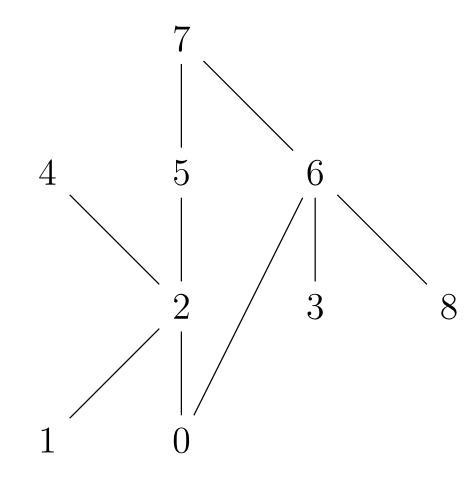
\includegraphics[width=5cm]{img/hasse.png}
		\end{center}
		\caption{Hasse-Diagramm einer unbekannten Relation R auf eine Menge $[0,8]$}
		\label{fig:}
\end{figure}

\section{Unendlichkeiten}
Eine undenlich grosse Menge ist eine Menge, die endlos viele Elemente enthält. Allerdings ist das rechnen mit solchen Mengen kompliziert, das z.b. \(| \mathbb{N}| = |2 \mathbb{N}|\) wahr ist.
\subsection{Mächtigkeiten}
Unendlich grosse Mengen können in \textbf{abzählbar grosse} und in \textbf{überabzählbar grosse} Mengen unterteilt werden. Mit abzählbar grossen unendlichen Mengen sind Mengen gemeint, die mit den natürlichen Zahlen durch nummeriert werden können. Sprich es besteht eine \textit{Bijektivität} von \( \mathbb{N}\) zu dieser Menge. Beispiele für abzählbar unendlich grosse Mengen sind \( \mathbb{N}\), \( \mathbb{Z}\), \( \mathbb{R}\) aber auch kartesische Produkte wie \( \mathbb{N}\times \mathbb{N}\) oder \( \mathbb{R}\times \mathbb{R}\). Ein Beispiel für eine überabzählbar grosse Menge ist z.b. \( \mathbb{Q}\) oder demnach auch \( \mathbb{Q}\times \mathbb{Q}\). Eine Menge \(X\) ist genau dann überabzählbar, wenn eine Liste \(x_1\), \( x_2\), \(x_3, ...\) nie komplett ist.

\newpage
\subsection{Cantor}
Georg Cantor war ein deutscher Mathematiker, der mit seinen zwei Diagonalargumenten bewiesen hat, dass 1. \( \mathbb{R}\) abzählbar und 2. \( \mathbb{Q}\) überabzählbar ist.
\begin{center}
\begin{figure}[h]
		\begin{center}
		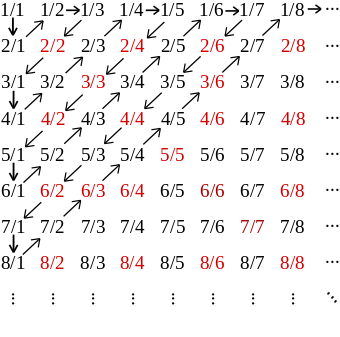
\includegraphics[width=5cm]{img/cantor1.png}
		\caption{erstes Diagonalargument}
		\label{fig:erstes Diagonalargument}
		\end{center}
\end{figure}
\end{center}
\begin{center}
\begin{figure}[h]
		\begin{center}
		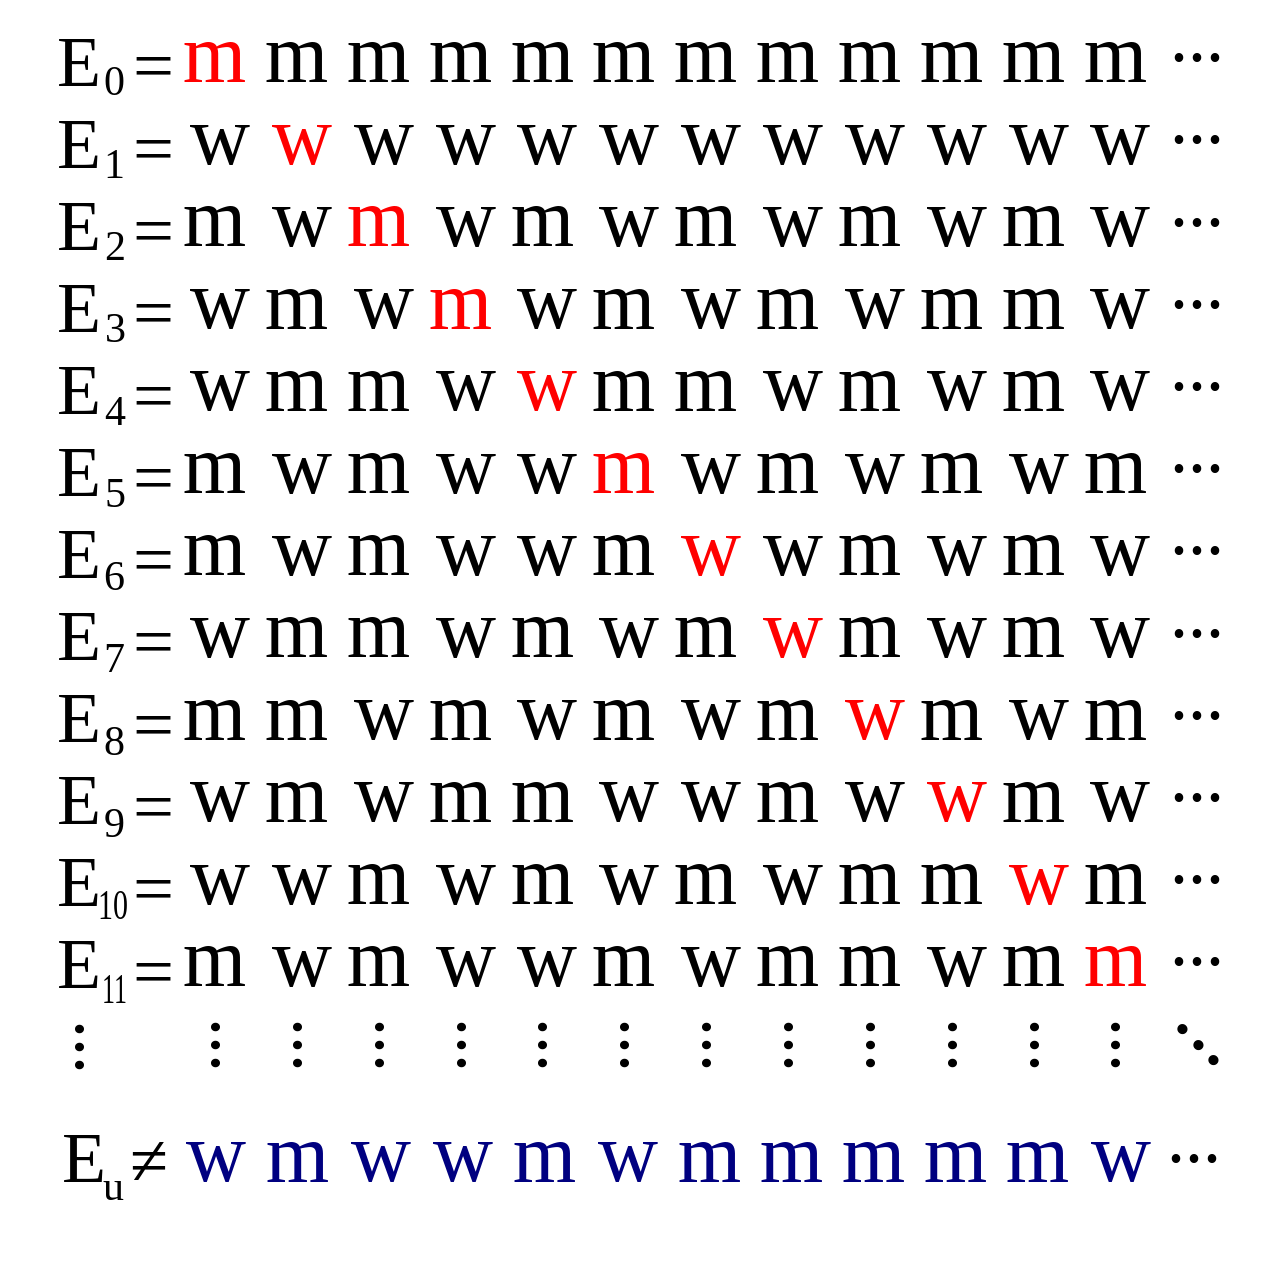
\includegraphics[width=5cm]{img/cantor.png}
		\caption{zweites Diagonalargument}
		\label{fig:zweites Diagonalargument}
		\end{center}
\end{figure}
\end{center}

\end{document}
